\documentclass{article}
\usepackage[a4paper, margin=1in]{geometry}
\usepackage{datetime}
\usepackage{graphicx}
\newdate{date}{24}{1}{2023}
\date{\displaydate{date}}

\usepackage{hyperref}
\usepackage{minted}

\title{Initiation to 3D Printing -- Practical exercises 2}
\author{Sylvain Lefebvre and Camille Schreck, ENSEM 2020-2021}

\begin{document}

\maketitle

\section{Important information}
\begin{itemize}
    \item I recommand to write the code in C++ (the templates and corrections will be in C++). But you can also use C, Python, or JAVA.
    \item At the end of the session, send the {\bfseries code and GCode of exercises 4, 5, 6 and 7}. The files should be in a single folder called {\bfseries TP1\_[nom][prenom]} and compressed into a ZIP (or tar.gz..) file to:
    \begin{itemize}
        \item \href{mailto:sylvain.lefebvre@inria.fr}{sylvain.lefebvre@inria.fr}
        \item \href{mailto:camille.schreck@inria.fr}{camille.schreck@inria.fr}
    \end{itemize}
    with the mail subject {\bfseries ENSEM: TP 1 [nom][prenom]}
\end{itemize}


\section{Useful Links}

\begin{itemize}
	\item To write and test GCode \url{https://icesl.loria.fr/webprinter/}\\ (older version: \url{http://shapeforge.loria.fr/vrprinter})
	\item Another GCode viewer \url{http://gcode.ws}
	\item List of GCode instructions \url{http://marlinfw.org/meta/gcode/}
\end{itemize}

\section{Exercise: filling the square (zigzag infill)}

\begin{enumerate}
    \item Consider a square with dimensions $40 \times 40$mm.
Implement the filling of the square (slice) with a zigzag infill. Make sure that the zigzag fills (as close as possible) 100\% of the inside of the square
Beware of overlaps!

\begin{center}
\includegraphics[width=0.3\linewidth]{zigzag.png}
\end{center}

\item Modify the program to output 50 layers of thickness 0.2mm, for an object of 10mm height in total. The zigzag main direction rotated 90 degrees at each slice (left/right, then front/back).
\end{enumerate}

\section{Exercise: filling the square (contour parallel infill)}

\begin{enumerate}
    \item Consider again a square with dimensions $40 \times 40$mm.
Implement the filling of the square (slice) with a contour parallel infill.

\begin{center}
\includegraphics[width=0.3\linewidth]{contourparallel.png}
\end{center}

\item Modify the program to output 50 layers of thickness 0.2mm, for an object of 10mm height in total.
\end{enumerate}

\section{Exercise: mixing zig zag and contour parallel}

\begin{enumerate}
\item Consider again square with dimensions $40 \times 40$mm.
Implement the filling of the square with two parallel contours, followed by the zig-zag infill.
\item Modify the program to output 50 layers of thickness 0.2mm, for an object of 10mm height in total.
\end{enumerate}

\section{Exercise: filling the hemisphere}

\begin{enumerate}
\item Implement a program outputting the GCode of of circle of 20mm radius on one layer. It will be filled with two contour parallel tracks, followed by a zigzag infill.
\item Bonus: Implement a program outputting the GCode of an hemisphere of 20mm radius with 0.2mm layers. Each layer will be filled with two contour parallel tracks, followed by a zigzag infill.
\end{enumerate}

\section{Sparse filling a cube}

\subsection{Three sets of parallel lines in a square}

We are going to fill a square of $36 \times 36$ mm with three sets of parallel lines:

\begin{enumerate}
\item The first set is at a $45$ degree angle with a spacing of 4mm.

\begin{center}
\includegraphics[width=0.1\linewidth]{45deg.pdf}
\end{center}
\item The second set is at a $-45$ degrees angle with a spacing of 4mm.

\begin{center}
\includegraphics[width=0.1\linewidth]{315deg.pdf}
\end{center}
\item The last set is at an angle of $0$ degree angle with a spacing of 4mm.

\begin{center}
\includegraphics[width=0.1\linewidth]{0deg.pdf}
\end{center}
\end{enumerate}

Make sure the 4mm spacing can be adjusted from a variable.


\subsection{Progressive offset in the cube}

We are going to fill a cube of dimensions $36 \times 36 \times 36$ mm

Progressively offset the lines at each layer, moving them sideways (to their right) by half a nozzle (typically 0.2mm). Generate GCode. You should now see three sets of angled walls forming closed 3D cells. For an illustration and more information refer to this URL:

\url{http://sylefeb.blogspot.com/2015/07/3dprint-3d-infilling-faster-stronger.html}

\begin{center}
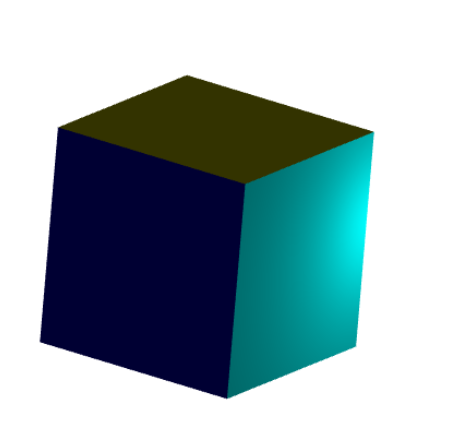
\includegraphics[width=0.25\linewidth]{cube.jpeg}
\end{center}


\section{Miscellaneous: sample code C++}

\begin{minted}{cpp}
#include <iostream>
#include <fstream>
#include <cmath>  // use constant M_PI to get the value of pi

int main () {
    std::ofstream file;
    file.open ("square.gcode");
    // header
    file << "G21" << std::endl;  // dimensions in milimeters
    file << "G90" << std::endl;  // absolute positioning
    file << "G28" << std::endl;  // homing

    // exercise code
    file.close();
    return 0;
}

\end{minted}

In Linux, compile the above program (contained in a file main.cpp) with:

\begin{minted}{bash}
g++ main.cpp -o main
\end{minted}

\end{document}

